\documentclass[12pt]{article}
\usepackage{graphicx}
\usepackage[spanish]{babel}
\usepackage{graphicx}

\title{Proyecto de Tesis}
\author{César Humberto Estrada Crisanto \\
PROGRAMA DE DOCTORADO EN CIENCIAS \\ CON MENCION EN ENERGETICA \\
Universidad Nacional de Ingenieria}
\date{25 marzo 2023}

% inicia el documento
\begin{document}
	\maketitle
	
\begin{abstract}
	
	

\end{abstract}

%coloquemos el indice
\tableofcontents

%obliguemos a un salto de pagina
\newpage
	
\section{Area de Investigación}
Electronica de Potencia - Electromovilidad	


\section{Titulo del trabajo Propuesto}
Análisis de rendimiento y diseño de vehículos eléctricos fotovoltaicos alimentados por pilas de combustible

\section{Problema de Investigacion}
En la literatura, varios convertidores CC-CC de entrada múltiple con ganancia de alto voltaje y convertidores CC-CC bidireccionales están disponibles para aumentar las fuentes de energía renovable de bajo voltaje al nivel requerido y para que el flujo de energía sea bidireccional en la batería , es decir para los modos de carga y descarga, operando en su ciclo de trabajo máximo, lo que aumenta la tensión de conmutación y reduce el rendimiento del convertidor DC-DC. De manera similar, para obtener el punto de máxima potencia, muchos algoritmos de control MPPT están disponibles en la literatura. Cada algoritmo MPPT tiene sus propias ventajas y desventajas.
\begin{figure}[h]
	\centering
	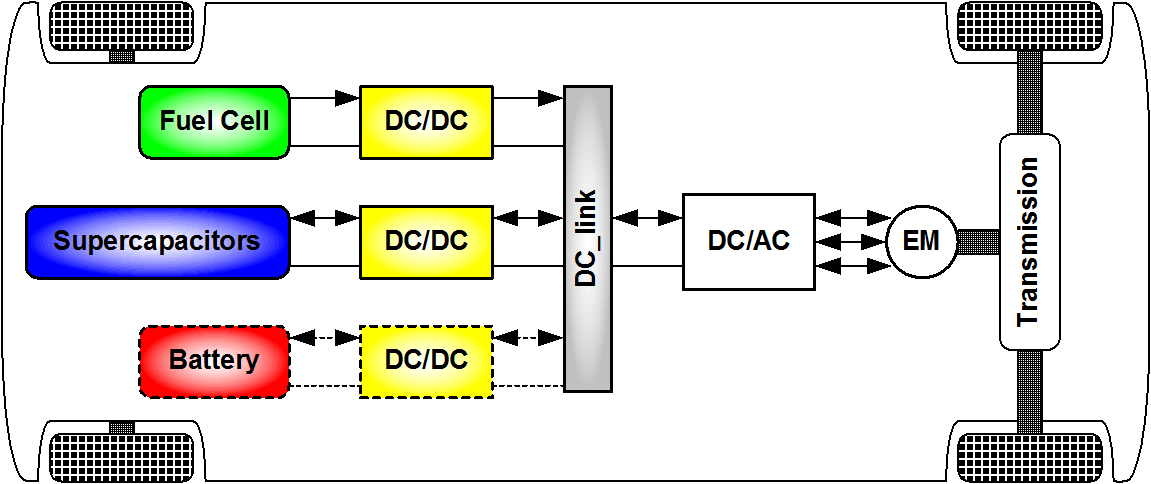
\includegraphics{image2.png}
	
	
\end{figure}

\section{Novedad de Investigacion}
Diseño de convertidores DC-DC de alta ganancia y convertidores bidireccionales adecuados para vehículos eléctricos alimentados con celdas de combustible y fotovoltaicos.

\section{Introduccion}
La filosofia del nuevo auto electrico deriva de varios factores los cuales incluye avances en tecnologia, cambio de habitos de los usuarios, el incremento de la conciencia ambiental y una necesidad general de dar una nueva mirada radical al futuro de la movilidad[1]
Existen diversos modelamientos para realizar la evaluacion y el rendimiento de un vehiculo hibrido, de los cuales existen dos herramientas: estado estacionario y herramientas dinamicas, en esta referencia se realizo el segundo que incluyen muchos componentes como: motor electrico, baterias, generador y su maquina de combustion, el trabajo incluye simulacion usando el ADVISOR (ADvanced VehIcle SimulatoR).[2]
Con respecto a los conversores bidireccionales tiene significante interes y aplicaciones en vehiculos electricos. Para un conversor DC-DC bidireccional , una bateria, la cadena de traccion y el motor son excitados por separado. Este convertidor y controlador realiza el trabajo de aceleración y presión para igualar el voltaje nominal de la batería del motor para controlar la situación de frenado del flujo de energía.
la aceleración , modo normal del motor, y la energía cinética del motor se convierte en energía eléctrica fluye entre la energía de la batería durante el modo de frenado o regenerativo y se retroalimenta a la batería[3]






\section{Objetivo}
\begin{itemize}
	\item Identificar convertidores de CC-CC de ganancia de alto voltaje adecuados y convertidores de CC-CC bidireccionales con operación de ciclo de trabajo mínimo para sistemas de vehículos eléctricos alimentados con pilas de combustible y fotovoltaicos.
	\item Desarrollar un controlador MPPT inteligente con sistema de gestión de energía para aplicación en vehículos eléctricos híbridos.
\end{itemize}




\section{Metodologia}
Trabajar en la literatura para encontrar el mejor y más apropiado convertidor adecuado para la aplicación de vehículos eléctricos híbridos. \\ En este estudio de investigación propuesto, un convertidor CC-CC de ganancia de alto voltaje adecuado y convertidores CC-CC bidireccionales con operación de ciclo de trabajo mínimo para sistemas de vehículos eléctricos alimentados con celdas de combustible y FV y un controlador MPPT inteligente con sistema de administración de energía son los dos objetivos principales de el trabajo de investigación propuesto.


\section{Resultados Finales}
\begin{itemize}
\item Obtención de convertidores DC-DC  bidireccionales de alta ganancia adecuados para aplicaciones de vehículos eléctricos.
\item Presentar un modelo competitivo de vehículo eléctrico híbrido.
\item Publicar un buen número de artículos de investigación.



\end{itemize}


%fin del documento


\section{Referencias}
\begin{itemize}
\item [1] Making of an 'all reason' electric vehicle, autor: Chetan Maini, Kartik Gopal,R Prakash, Bangalore 2013    
\item [2] Modeling and Simulation of Electric and Hybrid Vehicles for Recreational Vehicle, autor: Mohamed YAICH, Moez GHARIANI, Mohamed Radhouan HACHICHA, Tunisia 2015
\item [3] A bidirectional DC-DC converter fed separately excited DC motor electric vehicle application, autor: Amit Tanaji Waghe, dR S.K. Patil, Karad, 2020






\end{itemize}









\end{document} 